\chapter{Results and Discussion}
\label{chapter:results_and_discussion}

This chapter presents and discusses the results that we found through analyzing the collected data (see \autoref{table:data}), results from the semi-structured interviews, and findings from the two questionnaires.

\section{Usability}
\label{section:usability}
%  more info on usability score: https://measuringu.com/sus/
% A SUS score above 68 would be considered above average, and anything below 68 is below average.
% # A SUS score of 74 has higher perceived usability than 70\% of all products tested. It can be interpreted as a grade of a B-.

The results from the usability questionnaire which the participants answered at the end of the study are shown in \autoref{fig:usability_questionnaire}. For the questions with even numbers, e.g., Q2, Q4, etc., negative answers are desirable, whereas, in questions with uneven numbers, e.g., Q1, Q3, etc., positive, blue responses are ideal. Generally, the result looks very promising. There are, however, some answers worth discussing. The \enquote{disagree} answer from Q1 came from P586. P586 also disagreed that the various functions of the application were well-integrated (Q5). The reasons for these answers could be found in the interview, where the following statement was made.

\begin{displayquote}
    Uhm, as a separate tool, I would not use it. Integrated into another communication tool, I might use it, yes. -P586
\end{displayquote}

The \enquote{agree} response in questions Q4 and Q10 came from P163, indicating that the number of featured in AmbientTeams is quite demanding to understand simply during the initial meeting. Nevertheless, this participant did not mention any usability issues in the interview nor through direct feedback, leading us to believe that it was straightforward to use after the initial challenge of understanding the application.

\begin{figure}[h]
    \centering
    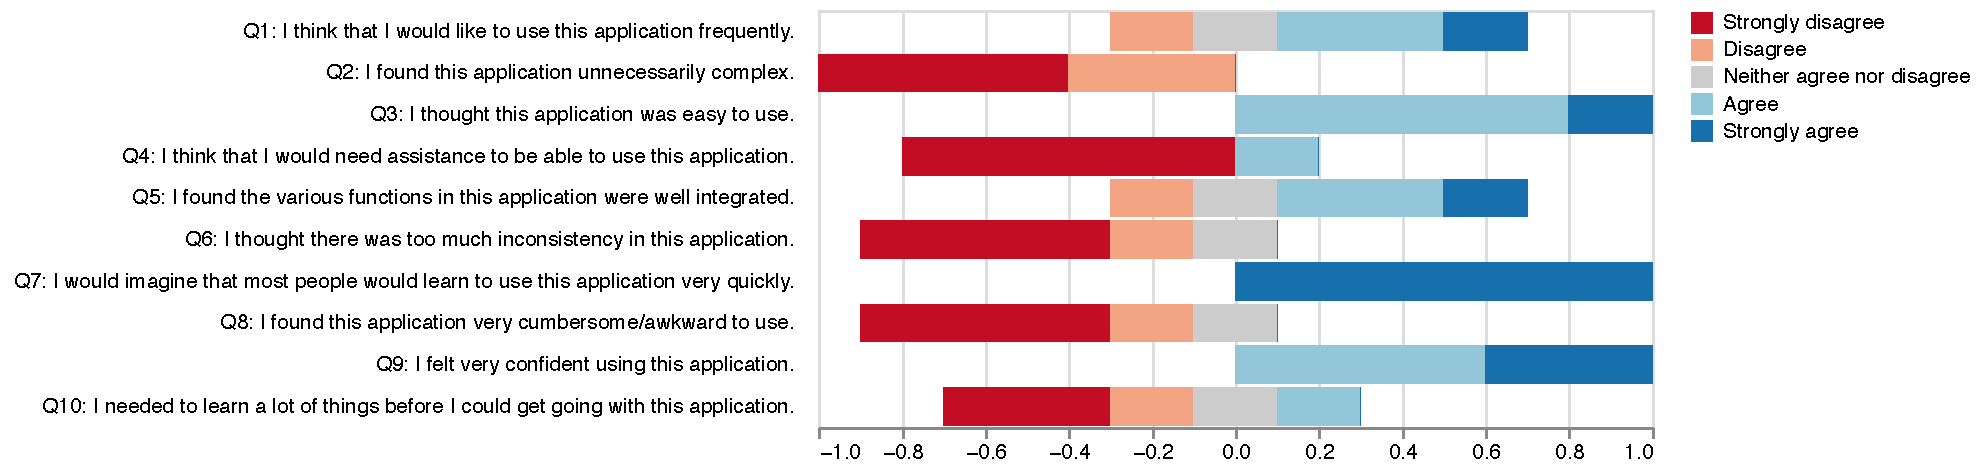
\includegraphics[width=\linewidth]{plots/usability_likert.pdf}
    \caption{Usability questionnaire results}
    \label{fig:usability_questionnaire}
\end{figure}

The individual participants' answers were then converted into the SUS score for each question according to \textcite{sauroSUS} to get a comparable score. The resulting average SUS score was 81.1 across all five participants (see \autoref{table:sus}). According to \textcite{sauroSUS}, one would need to score above 80.3 to be in the top 10\% of the 500 studies using the SUS. 80.3 is also the point where users are more likely to be recommending the product to a friend \autocite{sauroSUS}, making us believe that AmbientTeams was easy and intuitive to use.

\begin{table}[h]
    \centering
    \begin{tabular}{|l | l|}
        \hline
        Participant & SUS score \\
        \hline
        P038        & 82.5      \\
        % \hline
        P163        & 80.0      \\
        % \hline
        P586        & 70.0      \\
        % \hline
        P751        & 82.5      \\
        % \hline
        P904        & 90.5      \\
        \hline
        Average     & 81.1      \\
        \hline
    \end{tabular}
    \caption{Usability questionnaire results and resulting SUS score}
    \label{table:sus}
\end{table}

\section{Tool Usage and Workflows (RQ4)}
\label{section:tool_usage_and_workflows}

A detailed timeline view of the participants and their selected availability state (\enquote{Available}, \enquote{Focused}, or \enquote{Happy to interact}) throughout the study is visualized in \autoref{fig:non_offline}. Those three states combined are looked at as the time when the application was running (potentially in the background). This is because the user is automatically set to an offline state if the connection to the server is lost. Upon successful connection to the server, the user's availability state is also automatically set to \enquote{Available}. It is worth mentioning that this metric could be slightly erroneous if participants manually set their availability status to \enquote{Offline}. This would, however, only underestimate the time spent online in \autoref{fig:non_offline}, making our results as conservative as possible. All in all, the average time spent in a non-offline state, and thus AmbientTeams was running (potentially only in the background), was 7.13 hours per day (std. 3.57), with a minimum of 0 and a maximum of 12.7 hours. Except for the inactivity on the weekend, only some participants did not use AmbientTeams some days. To be precise, only 5 out of a total of 30 workdays showed no or very short running time. The fact that P038 could not participate in the initial meeting with the rest of the group explains the lack of usage on the first day of the study. In general, because the kick-off meeting took place in the early afternoon, the relatively short running time on the first day was to be expected. The remaining days with very little only time most likely indicate non-working days for those participants because had they worked on those days, AmbientTeams would have automatically started as soon as they had started up their computer.

\begin{figure}[h]
    \centering
    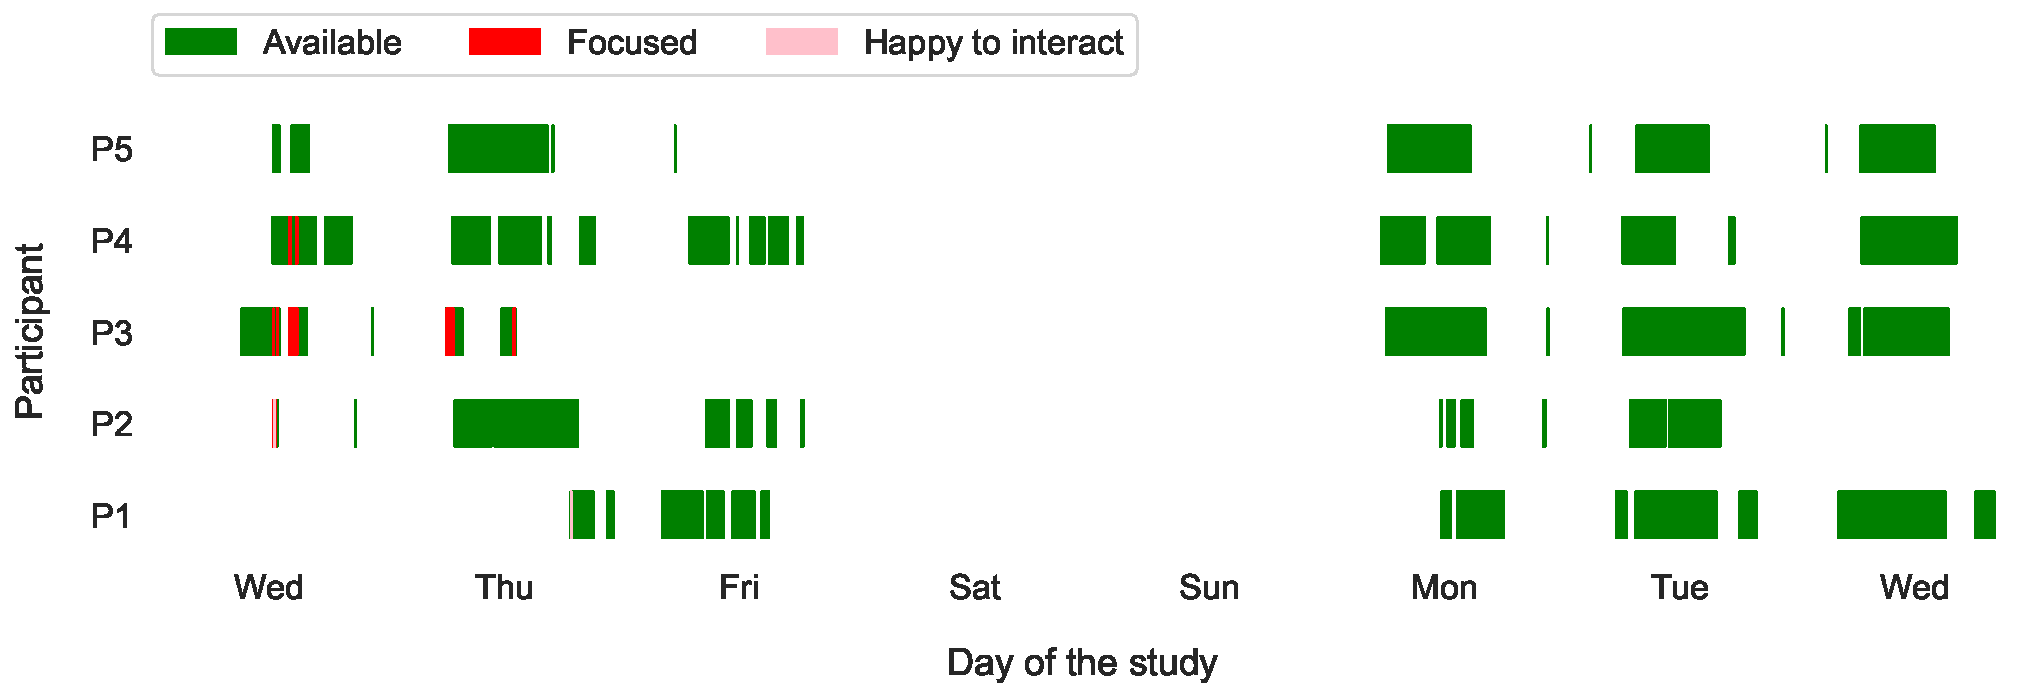
\includegraphics[width=\linewidth]{plots/non_offline.pdf}
    \caption{Time spent in the different availability states}
    \label{fig:non_offline}
\end{figure}

The results show that the participants did not often change their availability states and thus mainly relied on the automatic availability status setting of AmbientTeams. The \enquote{Focused} state was selected a couple of times in the first two days of the study, yet this behavior did not continue throughout the study.

\subsection{Challenges and Novelty of the Ambient Window}
\autoref{fig:opened_vs_focused} illustrates that both the ambient window and the team overview window were almost exclusively opened when those windows were in focus. In other words, both of those windows were opened, interaction took place, and then they were closed or minimized again, making them disappear from the user's monitor. This is the result we expected to happen in the case of the team overview. In contrast to our beliefs, however, the ambient window was used very similarly. As a result, the ambient window only very rarely was kept open as a glanceable, always-on-top team view when working on other tasks.

\begin{figure}[h]
    \centering
    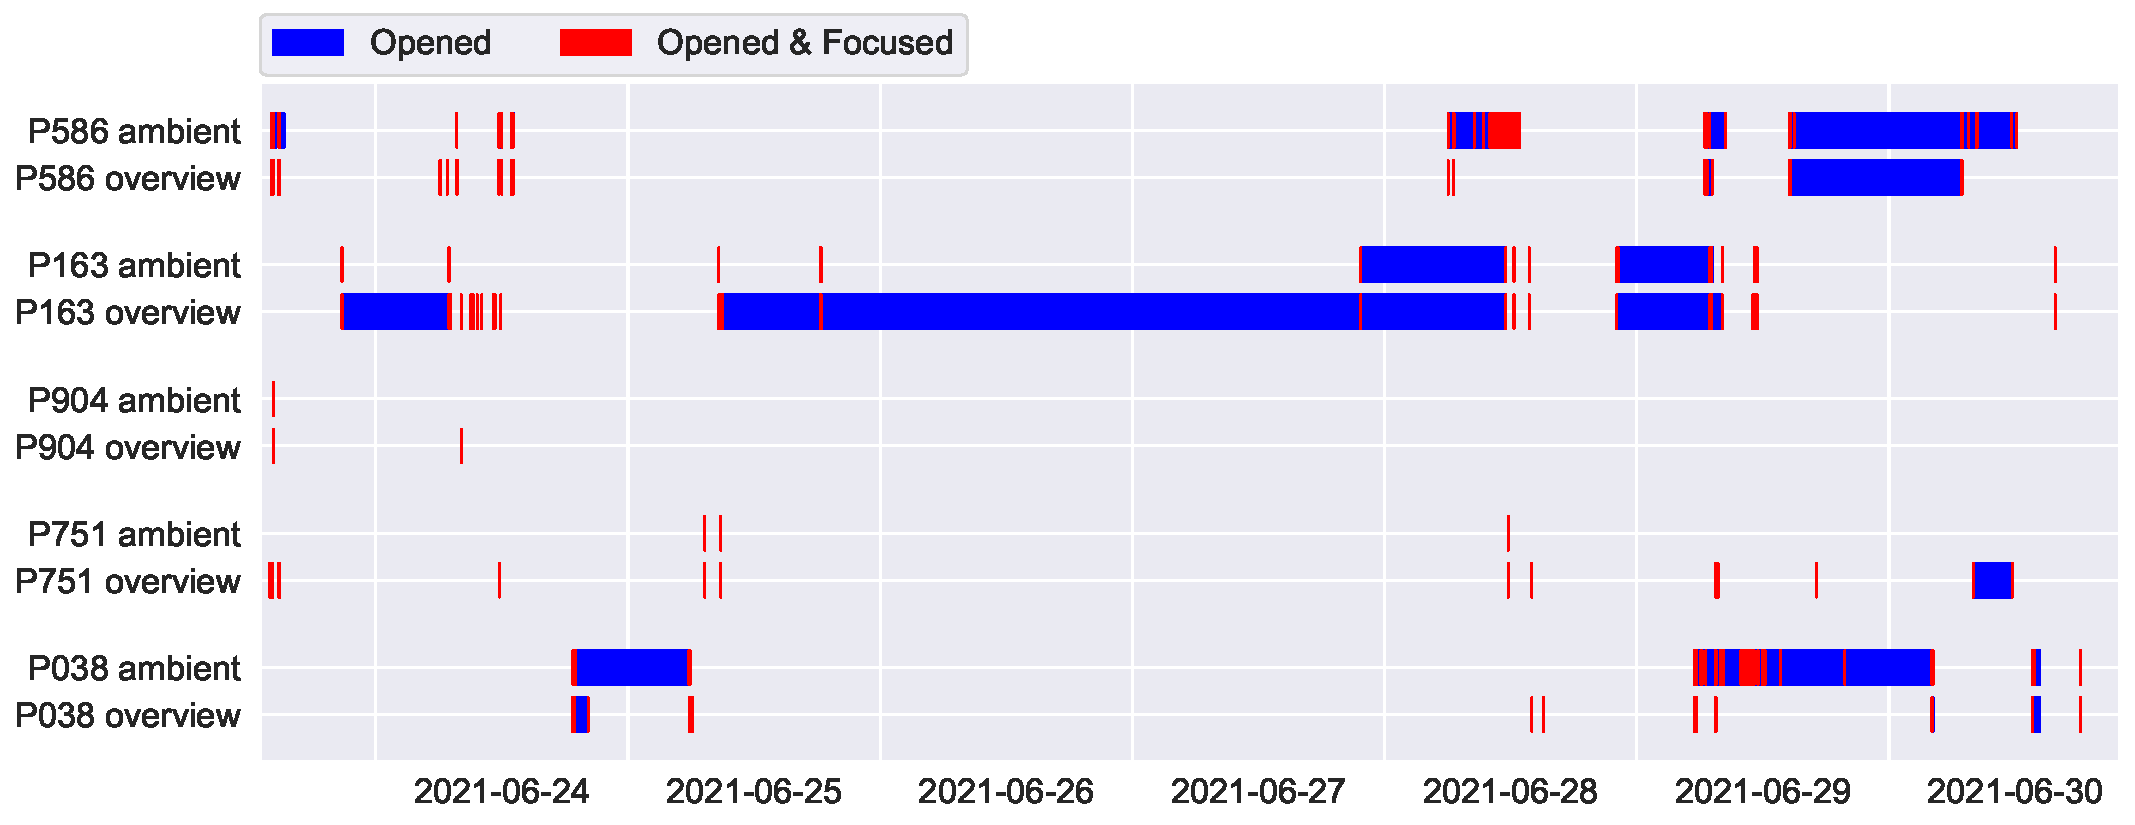
\includegraphics[width=\linewidth]{plots/open_vs_focus.pdf}
    \caption{Time AmbientTeams was opened vs. opened and focused}
    \label{fig:opened_vs_focused}
\end{figure}

The interviews gave us some more insights into possible answers for why the ambient window was not kept open while working on other tasks.

\begin{displayquote}
    I tried it in the corner of the monitor, then it did not work, but in the corner of the window did not really work because there you have to click to close other windows. Then I put it somewhere in the middle, but then I needed to put some buttons there, so sometimes I got annoyed and then closed it. -P038
\end{displayquote}

We hypothesize that this particular user most likely was using a single monitor setup and had a hard time finding a suitable position for the ambient window. P586 mentioned that the ambient window was too small and thus too difficult to properly move around, indicating that this participant might have missed this part of the demonstration during the kick-off meeting. In addition to the annoyance of the ambient window experienced by P038 and P586, P163 mentioned that manually closing an application that automatically starts up is something that happens almost automatically to them because of established habbits. The hassle and difficulties of positioning the ambient window are a rather crucial issue that potentially requires further development; the case described by P163 could be solved by not allowing to close the ambient window during a future study.

To make the ambient window fit better into their workflow, P038 suggested that it should ideally not stay on top of other windows and instead just come to the foreground again once a team member has shared something new. P586 similarly suggested that the ambient window ideally should fade out when not being used.

Despite the criticism around the ambient window, it was still used by all the participants except for P904 and seen as one of the best aspects of AmbientTeams by P751:

\begin{displayquote}
    I liked that the ambient window feels very dynamic and refreshing compared to other tools. -P751
\end{displayquote}

Despite this positive statement, this participant used the team overview window more, which is surprising because all the participants were only part of one team during the study, eliminating the potential advantage of the team overview window, in our opinion.

\section{A Need for Status and Mood Sharing (RQ1)}
From the interviews, we could identify two reasons why there is a need for mood sharing at the workplace: the lack of 1) awareness and 2) social interactions in remote work environments. This finding further confirms our motivation to create AmbientTeams in the first place.

\medskip\noindent\textbf{Lack of Awareness} \\
P163 explained that there is a lack of awareness of the \textit{real} mood when working remotely. Even though you might see them during video conferences, it makes the impression that feelings expressed through such calls might not be real.

\begin{displayquote}
    I think it's a good idea, especially now if you work either hybrid or completely remote, I think then it is quite difficult to see the mood of your team colleagues, because now in most video conferences you make a happy face into the camera, so it is also difficult to see your mood how your mood really is right now. -P163
\end{displayquote}

To highlight this point more, four out of five participants mentioned in the pre-study questionnaire that they are not or only partially aware of their co-workers' moods. This is because of missing cues resulting from working from home, according to P586.

\begin{displayquote}
    I like to ask people how they feel but being in a room with your colleagues gives you more information about how someone is actually feeling. -P586
\end{displayquote}

Those two statements both talk about the concept of honesty in regards to expressing feelings, a topic that was, unexpectedly, talked a lot about during the interviews and will therefore be covered in more detail in \autoref{section:negative_moods_and_honesty}.

But why is mood awareness important? Being aware of your co-worker's feelings is essential for personal relationships, something important, says P751.

\begin{displayquote}
    Yes, it [feeling of co-workers] is important to me because if you think about how much time you spend with your co-workers, it is very important that you have good personal relationships with those people. Even when it's not clear how much longer you will be working together with those people. -P751
\end{displayquote}

In addition, certain conclusions about the current workload of employees can also be drawn through the exchange of moods and states, facilitating task assignment.

\begin{displayquote}
    Sometimes I then [at a previous company] got the feedback that they already finished with work or that they have no more tasks left. With something like AmbientTeams they could set like a bored state, and I would have been able to give them a new task. -P163
\end{displayquote}

\medskip\noindent\textbf{Lack of social contact / task-focus} \\
One participant (P032) talked about how working remotely often is very task-centric, which leads to forgetting about the \enquote{social aspects of an enterprise}. P586 mentioned that when working remotely, communication often is limited to be very business-focused, and conversations are therefore usually only started for business reasons.

\begin{displayquote}
    I think during corona, you don't really have that breakroom time, so if you call somebody, it's mostly about business and not about private stuff. So, I think it's very difficult to get into a deeper connection with people you don't see that often. -P586
\end{displayquote}

To conclude, there appears to be a need for some mood and status awareness-providing approach. The following sections look into how our approach, AmbientTeams, performed at tackling the challenges mentioned above.

\section{Moods Were Shared the Most  (RQ2)}
Moods were the most actively shared states, with a total of 31 moods being shared. In contrast, only eight status messages were shared, three of which were in reaction to Switzerland's soccer game during that time. Generally speaking, none of the status messages contained any work-related information.

\begin{figure}[h]
    \centering
    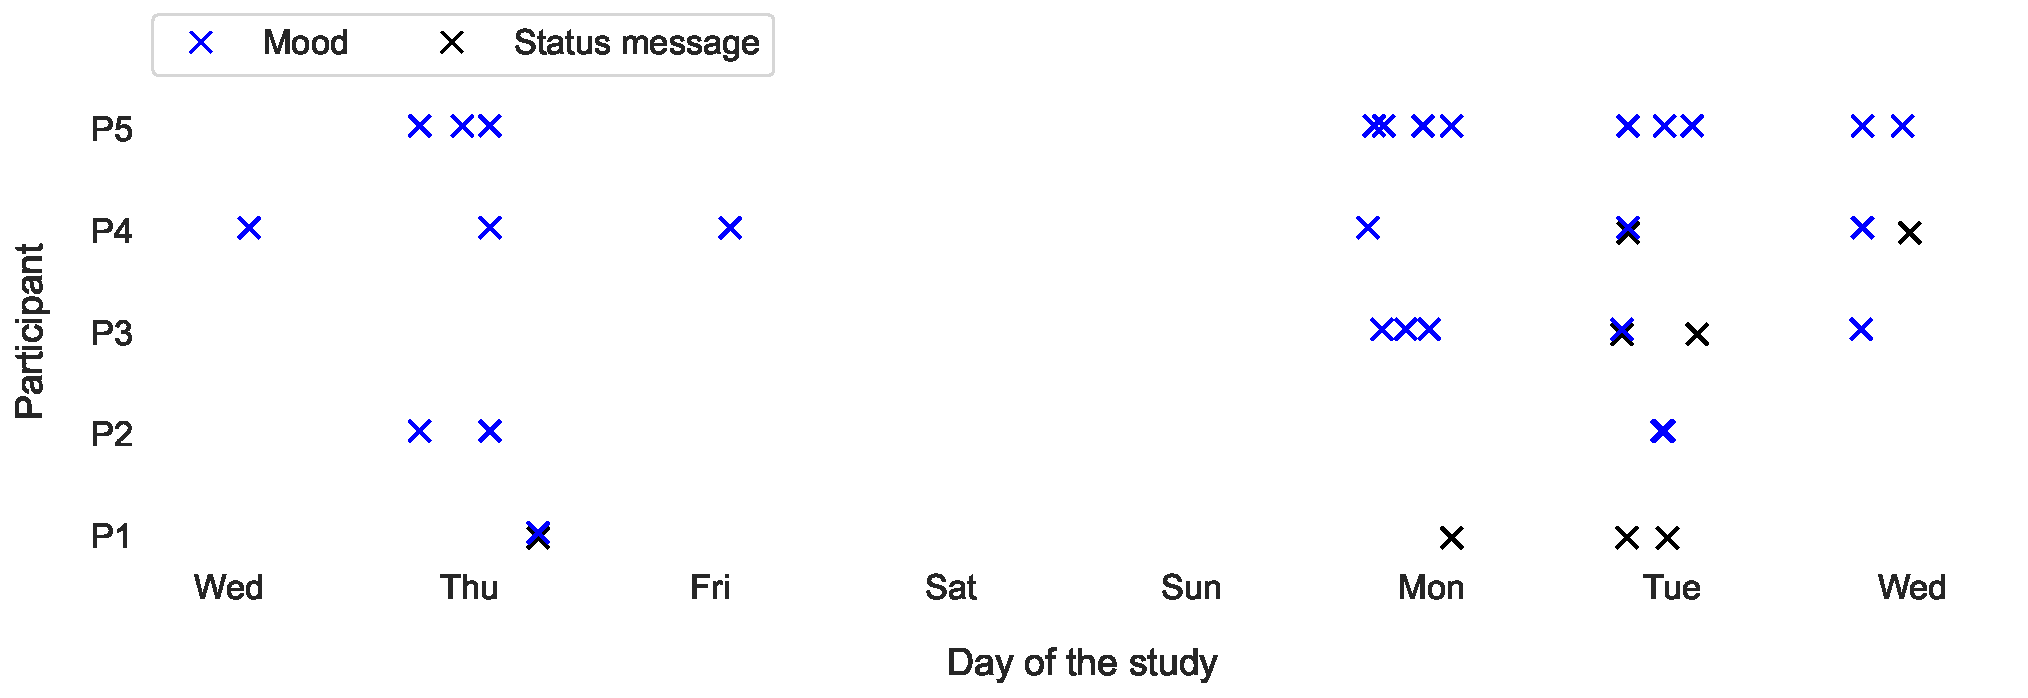
\includegraphics[width=\linewidth]{plots/moods_status_messages.pdf}
    \caption{Moods and status messages shared}
    \label{fig:moods_status_messages}
\end{figure}

Looking at \autoref{fig:moods_status_messages} shows that in only three cases, moods and status messages were shared simultaneously. According to the interviews, a primary reason for sharing moods was the automatically scheduled popup, which helped to remind the participants to share something. The data confirm this finding; 25 of the 32 shared moods were shared through the scheduled popup window. However, the participants usually just shared the mood through an emoticon and did not attach a text message. From P163, we learned that a potential reason could be that it was simply a lot quicker only to share the mood via emoticon, requiring only one click. P904 also mentioned that he/she did not see a reason to provide any more information to their mood (which was \enquote{tired} ten out of 12 times). TODO: Check if all three were negative.

While the scheduled popup helped remind the participants about sharing something, the motivation to share moods seemed to be that they knew the importance of communicating moods or interacting with co-workers (Pxxx). P586 also described how knowing that co-workers share the same feeling increases the likelihood of sharing this feeling yourself.

\begin{displayquote}
    And just this thing that I said before, if you have something that you are very happy about, you think that other people also share, then you are more motivated to share it as well. -P586
\end{displayquote}

% \begin{displayquote}
%     If we were not in a test phase, maybe I would not share that much if I saw that the others are also not really sharing anything. \\
%     -P586
% \end{displayquote}

Considering the relatively short time AmbientTeams was actively used, it is not surprising that many of its features were not used. More concretely, the features aimed at spontaneous interactions such as the breakroom and the random pairing for a video call were not used at all. While there have been two attempts of creating a breakroom, one on the second day of the study and one on the second to last day, none of them were successfully created because no other team member joined. P586 gave a possible explanation for why the spontaneous video chat features were not used during the interview.

\begin{displayquote}
    But also maybe I have to mention that two or three weeks ago we started with virtual break rooms on Friday afternoons to try to keep up with people from work, especially for new people, because we don't really get the chance to get to know each other in home office. -P586
\end{displayquote}

Consequently, it is possible that it is sufficient for the participating teams to meet once a week in their own virtual break room. Regardless of the use of the break room integrated into AmbientTeams, this indicates that the concept of such a break room is generally perceived as important. Similar to the breakroom, the directed video calls and the nudging functionality were only used during the initial kick-off meeting for testing purposes. While this shows that it was clear to the team how to use those features, they don't seem to have felt the need for those.

Things look a bit different when analyzing the direct messages that were sent through AmbientTeams. In total, there were six direct messages sent through AmbientTeams, coming from three different participants. One of those direct messages was a response to a missed call, and the other five were of either of type greeting or along the lines of \enquote{what are you doing?}. P032 gives an indication to why the team did not use the above-described functionalities:

\begin{displayquote}
    Because now it's a bit, you know I can write to somebody in Microsoft Teams or AmbientTeams, and I would normally pick MS Teams because we use it, and you also have a message history which you don't have in AmbientTeams. -P032
\end{displayquote}

Essentially, P032 explains that AmbientTeams has to differentiate itself from MS Teams, and it is doing so with the \textit{Twitter approach} of broadcasting moods and messages, but not so much with other communication functionalities.

\section{Negative Moods and Honesty (RQ2)}
\label{section:negative_moods_and_honesty}

When looking at \autoref{fig:moods_distribution}, it becomes apparent that, except for P904, who pretty much constantly was \enquote{Tired}, the most frequently shared moods were positive (especially \enquote{Happy}).

\begin{figure}[h]
    \centering
    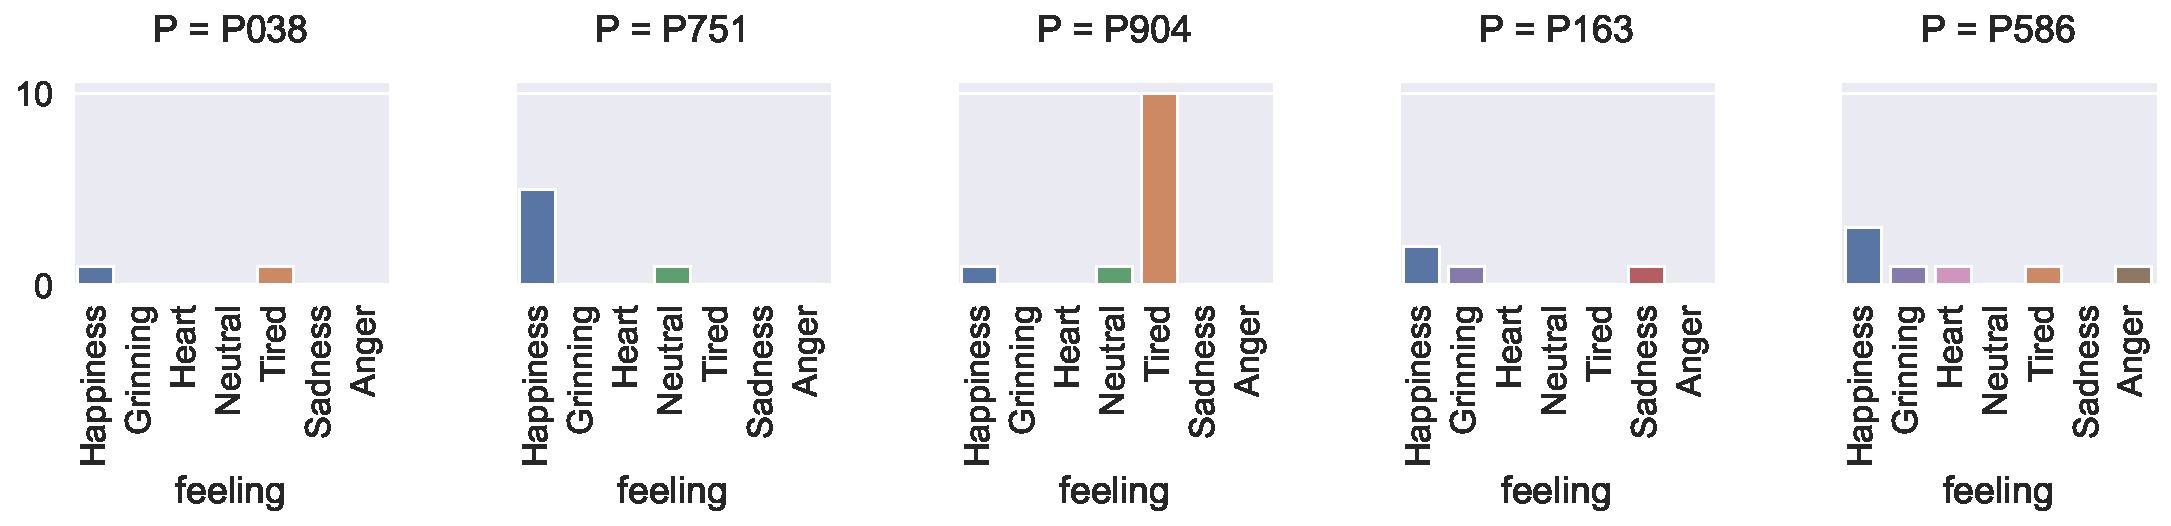
\includegraphics[width=\linewidth]{plots/moods_distribution.pdf}
    \caption{Distribution of shared moods }
    \label{fig:moods_distribution}
\end{figure}

Therefore, this finding raised the question, whether this was the real distribution of moods during the study or whether there could be a positive bias in moods when sharing. While P038 does not see a problem with sharing negative moods, because it's \enquote{normal, we are not in a happy boat where everyone is happy all the time}, others (P163, P586, P163) would be more hesitant to share such moods. Reasons for not sharing negative moods include 1) not wanting to give further explanations, either for private reasons or not wanting to be distracted (P163), 2) being fairly new to the company (P751), 3) not wanting to share them with the entire team (P586), or 4) because nobody wants to talk about negative feelings at work (P586).

% \begin{displayquote}
%     Yes, I think then it would be harder to share an angry mood. And if you are mad for private reasons, you maybe don't want to explain more. \\
%     -P163
% \end{displayquote}

% \begin{displayquote}
%     I would not share those things, like when I am tired or angry. \\
%     -P586
% \end{displayquote}

P751 further differentiates between the severeness of the experienced moods:

\begin{displayquote}
    I don't think I would share regular negative moods when having a bad day, for instance, being this new to a company. If something really severe were to happen, however, let's say something personal or family-related, I would share such moods to inform other people. -P751
\end{displayquote}


% \begin{displayquote}
%     But I always said that at this time that I had a good mood, this time this was honest, but I am not sure whether I would also share it if one day I had a bad mood. I am not sure if I then would be that honest to share it then directly online. \\
%     -P163
% \end{displayquote}

% -> Potentially undesired interruptions

% \begin{displayquote}
%     First reason is if I make, for example, an angry or sad mood, then everyone would text me, and I think I will maybe lose my focus because they would ask me why I was feeling in this way etc. And I think the second reason is that in the online world it is a lot easier to hide bad feelings, and you try to present yourself in the best way. \\
%     -P163
% \end{displayquote}

% \begin{displayquote}
%     It's easier to share positive feelings within a working environment compared to negative feelings because nobody wants to talk about negative feelings. \\
%     -P586
% \end{displayquote}

% While P586 also claims that talking about feelings is very important, sharing such personal information is not something that he/she likes to do.

% \begin{displayquote}
%     I mean of course it is very important that you talk about these kinds of things [feelings], but you don't want to share it with the whole team. \\
%     -P586
% \end{displayquote}

\section{Increased Awareness of Who Is Around and How They Feel (RQ3.1)}

The first effect of AmbientTeams was that participants learned who is around (P032, P586) and how they were feeling (P032, P751). P904 further noticed a key difference compared to their previous way of exchanging moods and feelings, which was usually done over text in the morning:

% \begin{displayquote}
%     Also, sometimes for just checking who is online and who is grayed out. -P586
% \end{displayquote}

\begin{displayquote}[][]
    [...] I wouldn't have known how you were doing during the day without AmbientTeams. [...] And, I think that's when you get additional information about how you're doing during the day. -P904
\end{displayquote}

This increased awareness had more implications, namely the possibility of getting to know each other better and bringing back a more natural way of communicating when working remotely. We will elaborate on both in the next sections.

\section{Getting to Know Each Other Better (RQ3)}
AmbientTeams allowed one person in particular

\begin{displayquote}
    Yes, actually about one particular person in the team. I did not know that this person was so funny before using AmbientTeams. The fact that I got to know one person a lot better during this one week and also having non-work-related talks now already exceeds my expectations for the study, to be honest. -P751
\end{displayquote}

\begin{displayquote}
    I very much like the idea of sharing moods with the team. As we are becoming more aware on such a sensitive topic as mental health, this feature allows to discover more about your colleagues, and it sheds light to a part that we tend to keep only for ourselves. -P751
\end{displayquote}

\begin{displayquote}
    I think it was very interesting to see moods and states of team members with whom I might not be currently working together too closely. -P751
\end{displayquote}

\begin{displayquote}
    Not really, to be honest. I just had the confirmation that one team member is really just always very positive and too nice. -P586
\end{displayquote}

\section{Bringing Back Communication Triggers}

\begin{displayquote}
    So if you do it purposely, I think 1:1, but I actually found it if you share it with the whole team. Because sometimes people then come back to you that you don't expect. So I mean, sometimes you don't have a good mood and people see it and want to cheer you up. So this substitutes a bit that part of the office life. -P038
\end{displayquote}

\begin{displayquote}
    So, for example, I saw that somebody pushed \enquote{good morning}, then I thought \enquote{ahh okay I need to speak to this person about some topic}, so I called this person on MS Teams. -P038
\end{displayquote}

Reason: Lower barrier

\begin{displayquote}
    Yes, definitely. It provides a lot more opportunities to approach another. -P904
\end{displayquote}

\begin{displayquote}
    Because if you only have to click on the avatar of Zsuzi or Adelina to start a conversation. -P163
\end{displayquote}

Reason: Help offering

\begin{displayquote}
    I think in that study not. But if somebody would have set an angry or stressed mood I would have helped him/her, if my current knowledge allowed it. -P163
\end{displayquote}

In fact:

\begin{displayquote}
    I had more non-work-related communication, however, outside of AmbientTeams in our existing tool. -P751
\end{displayquote}

\section{Mood Awareness via Self-Reflection (RQ3.2)}

\begin{displayquote}
    But I think it impacted myself because you're always prompted to think about your own mood. -P751
\end{displayquote}

\begin{displayquote}
    But if you're maybe tired or neutral, then maybe a few hours later you realized, I'm actually not tired or not so neutral, but rather happy. -P904
\end{displayquote}

\begin{displayquote}
    If I had something that could then show me afterward that for example, every time I do something for IT I am very happy, then I can maybe try to seek more tasks in IT and find my potential in IT and my life itself to make any further education for instance. -P586
\end{displayquote}

\section{Potential to Reduce Workplace Isolation (RQ3.4)}
\label{section:workplace_isolation}
Big disclaimer! Only 1 week, 5 participants, and no control group

Our approach to more quantitatively measure workplace isolation

Show chart. This chapter could also be kind of a summary